%%%%%%%%%%%%%%%%%%%%%%%%%%%%%%%%%%%%%%%%%
% Focus Beamer Presentation
% LaTeX Template
% Version 1.0 (8/8/18)
%
% This template has been downloaded from:
% http://www.LaTeXTemplates.com
%
% Original author:
% Pasquale Africa (https://github.com/elauksap/focus-beamertheme) with modifications by 
% Vel (vel@LaTeXTemplates.com)
%
% Template license:
% GNU GPL v3.0 License
%
% Important note:
% The bibliography/references need to be compiled with bibtex.
%
%%%%%%%%%%%%%%%%%%%%%%%%%%%%%%%%%%%%%%%%%

%----------------------------------------------------------------------------------------
%	PACKAGES AND OTHER DOCUMENT CONFIGURATIONS
%----------------------------------------------------------------------------------------

\documentclass{beamer}

\usetheme{focus} % Use the Focus theme supplied with the template
% Add option [numbering=none] to disable the footer progress bar
% Add option [numbering=fullbar] to show the footer progress bar as always full with a slide count

% Uncomment to enable the ice-blue theme
%\definecolor{main}{RGB}{92, 138, 168}
%\definecolor{background}{RGB}{240, 247, 255}

%------------------------------------------------

\usepackage{booktabs} % Required for better table rules
\usepackage{caption}


%----------------------------------------------------------------------------------------
%	 TITLE SLIDE
%----------------------------------------------------------------------------------------

\title{Analisi esplorativa del tasso di suicidio annuale in diversi paesi su dataset WHO}

\subtitle{Tesina di Data Science for Health Systems}

\author{Paolo Speziali}

\institute{Ingegneria Informatica e Robotica \\ Curriculum Data Science}

\date{A.A. 2022/2023}

\titlegraphic{
\includegraphics[scale=0.23, bb= 0 570 500 300]{Images/logounipg2021.png}} % Optional title page image, comment this line to remove it


%------------------------------------------------

\begin{document}

%------------------------------------------------

\begin{frame}
	\maketitle % Automatically created using the information in the commands above
\end{frame}

%----------------------------------------------------------------------------------------
%	 SECTION 1
%----------------------------------------------------------------------------------------

\section{Introduzione} % Section title slide, unnumbered

%------------------------------------------------

\begin{frame}{Introduzione}
	\begin{itemize}
		\item \textbf{Suicidio}: atto intenzionale di terminare la propria vita.
		\item Il suicidio è una delle principali cause di morte nel mondo occidentale.
		\item Dati stabili a livello nazionale nel breve termine, predizione basata sui tassi passati.
		\item Studio sui cambiamenti globali nel tasso di suicidio (2000-2019) e confronto tra regioni del mondo e gruppi di paesi.
	\end{itemize}
\end{frame}

\section{Dataset} % Section title slide, unnumbered

%------------------------------------------------

\begin{frame}{Descrizione del dataset}
	\begin{itemize}
		\item Origine del dataset: World Health Organization (WHO).
		\item Titolo del dataset: "Age-standardized suicide rates (per 100,000 population)".
		\item Copre il periodo dal 2000 al 2019 e include dati per soggetti maschili, femminili e di entrambi i sessi.
		\item Standardizzazione per la distribuzione dell'età della popolazione del paese.
		\item Acquisizione dei dati da censimenti, registrazioni anagrafiche e analisi di certificati medici.
		\item Struttura originale: $10'980$ campioni, $34$ feature, molte con valori nulli o non rilevanti per l'analisi.
	  \end{itemize}
\end{frame}

\begin{frame}{Modellazione del dataset}
	\begin{table}
		\centering
		\begin{tabular}{|c|c|}
		  \hline
		  \textbf{Nome Originale} & \textbf{Nuovo nome} \\
		  \hline
		  ParentLocation & WorldRegion \\
		  SpatialDimValueCode & CountryCode \\
		  Location & Country \\
		  Period & Year \\
		  Dim1 & Sex \\
		  FactValueNumeric & Value \\
		  \hline
		\end{tabular}
	  \end{table}
	  \begin{itemize}
		  \item Successivamente, il dataset è stato ulteriormente modificato per avere un'unica entry per ogni anno relativo a un paese.
		  \item La feature "Sex" è stata suddivisa in tre diverse feature (Male, Female, Both), ognuna contenente il valore associato nel campo "Value."
	  \end{itemize}
\end{frame}

\begin{frame}{Struttura finale del Dataset}
	Il nostro dataset è ora composto da $3660$ campioni e $7$ feature.
	\begin{itemize}
		\item WorldRegion: area geografica secondo la WHO.
		\item CountryCode: codice a tre lettere maiuscole del paese.
		\item Country: nome del paese.
		\item Year: anno del dato.
		\item Male: tasso di suicidi maschile.
		\item Female: tasso di suicidi femminile.
		\item Both: tasso di suicidi di entrambi i sessi.
	  \end{itemize}
\end{frame}

\section{Analisi Esplorativa dei Dati (EDA)} % Section title slide, unnumbered

\begin{frame}{Descrizione dell'EDA}
	Faremo l'analisi dell'intero dataset e poi di quattro
	gruppi di soggetti a seconda dei loro valori
	Both per ogni anno (2014-2019):
	\begin{enumerate}
		\item Regioni globali (WR)
		\item Paese con PIL più alto per WR
		\item Paesi con tasso di suicidio più alto in assoluto
		\item Paesi con tasso di suicidio più alto per WR
	\end{enumerate}
\end{frame}

\begin{frame}{Il quadro generale - Distribuzione per sesso}
	\begin{columns}
		\column{0.5\textwidth}
			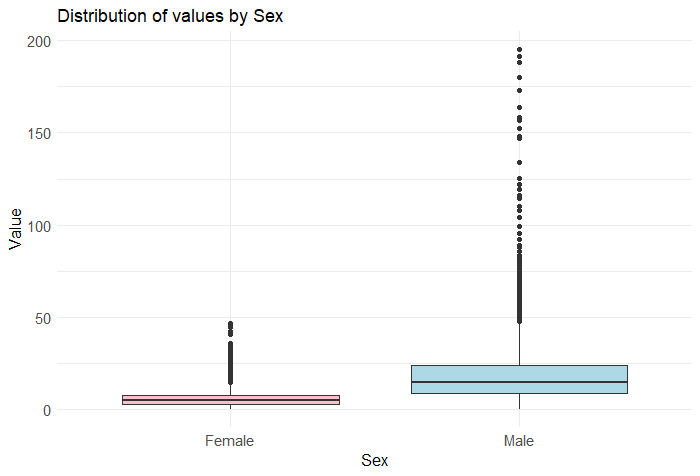
\includegraphics[width=\linewidth]{Images/1 - Sex2.png}
		\column{0.5\textwidth}
			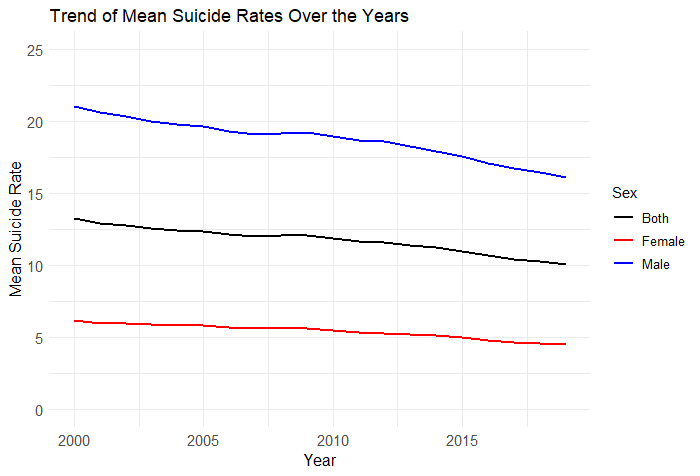
\includegraphics[width=\linewidth]{Images/2 - Globtrend2.png}
	\end{columns}
\end{frame}

\begin{frame}{Il quadro generale - Distribuzione per anno}
	\begin{columns}
		\column{0.5\textwidth}
			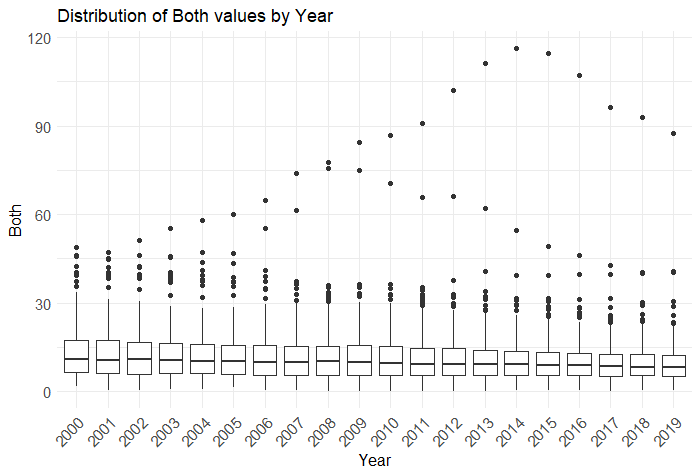
\includegraphics[width=\linewidth]{Images/3 - Boxyears2.png}
		\column{0.5\textwidth}
			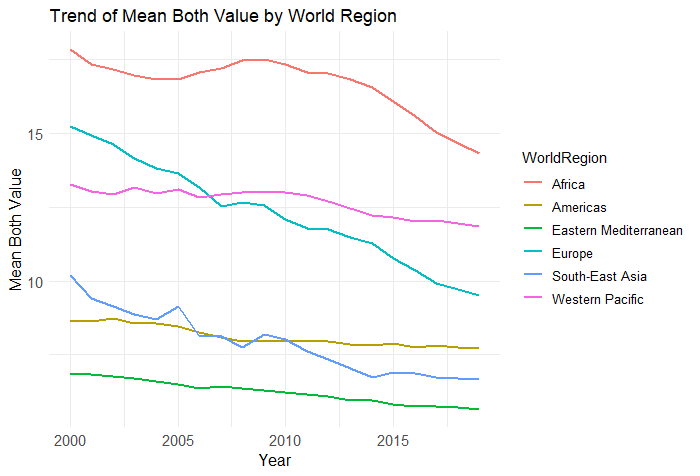
\includegraphics[width=\linewidth]{Images/4 - WRTrend2.png}
	\end{columns}
\end{frame}

\begin{frame}{Primo gruppo - Regioni globali}
	\begin{columns}
		\column{0.5\textwidth}
			\begin{itemize}
				\item \textbf{Africa}
				\item \textbf{Eastern Mediterranean}
				\item \textbf{Americas}
			\end{itemize}
			\bigskip
			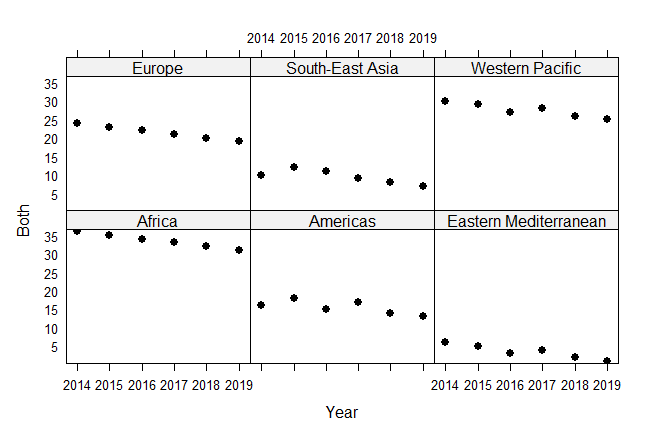
\includegraphics[width=\linewidth]{Images/5 - Firstgroup.png}
		\column{0.5\textwidth}
			\begin{itemize}
				\item \textbf{Europe}
				\item \textbf{Western Pacific}
				\item \textbf{South-East Asia}
			\end{itemize}
			\bigskip
			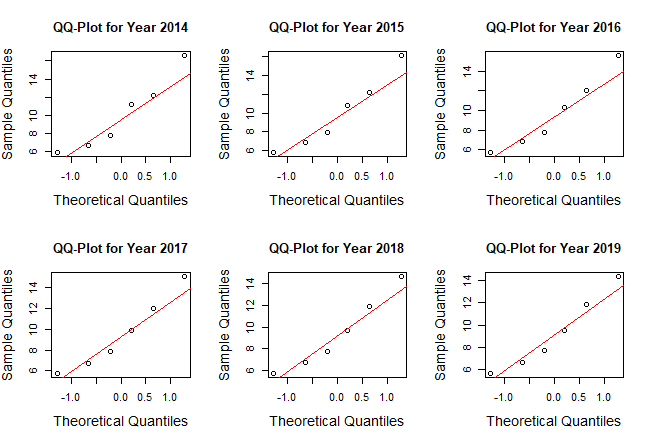
\includegraphics[width=\linewidth]{Images/6 - Firstqq.png}
	\end{columns}
\end{frame}

\begin{frame}{Secondo gruppo - Paese con PIL più alto per WR}
	\begin{columns}
		\column{0.5\textwidth}
			\begin{itemize}
				\item \textbf{Nigeria} (NGA) per Africa
				\item \textbf{Saudi Arabia} (SAU) per Eastern Mediterranean
				\item \textbf{United States of America} (USA) per Americas
			\end{itemize}
			\bigskip
			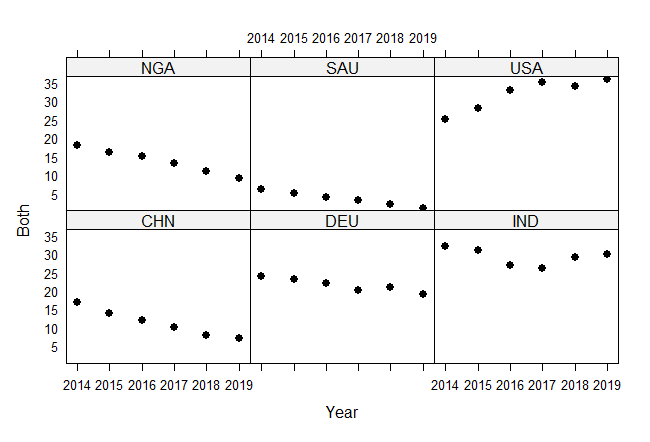
\includegraphics[width=\linewidth]{Images/7 - Secondgroup.png}
		\column{0.5\textwidth}
			\begin{itemize}
				\item \textbf{Germany} (DEU) per Europe
				\item \textbf{China} (CHN) per Western Pacific
				\item \textbf{India} (IND) per South-East Asia
			\end{itemize}
			\bigskip
			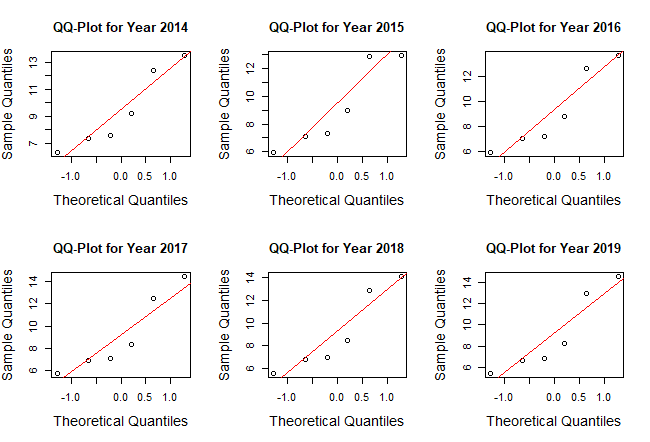
\includegraphics[width=\linewidth]{Images/8 - Secondqq.png}
	\end{columns}
\end{frame}

\begin{frame}{Terzo gruppo - Paesi con tasso di suicidio più alto in assoluto}
	\begin{columns}
		\column{0.5\textwidth}
			\begin{itemize}
				\item \textbf{Lesotho} (LSO)
				\item \textbf{Russian Federation} (RUS)
				\item \textbf{Eswatini} (SWZ)
			\end{itemize}
			\bigskip
			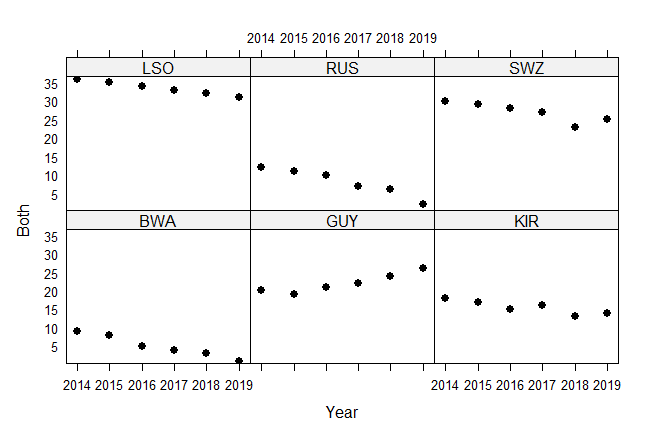
\includegraphics[width=\linewidth]{Images/9 - Thirdgroup.png}
		\column{0.5\textwidth}
			\begin{itemize}
				\item \textbf{Botswana} (BWA)
				\item \textbf{Guyana} (GUY)
				\item \textbf{Kiribati} (KIR)
			\end{itemize}
			\bigskip
			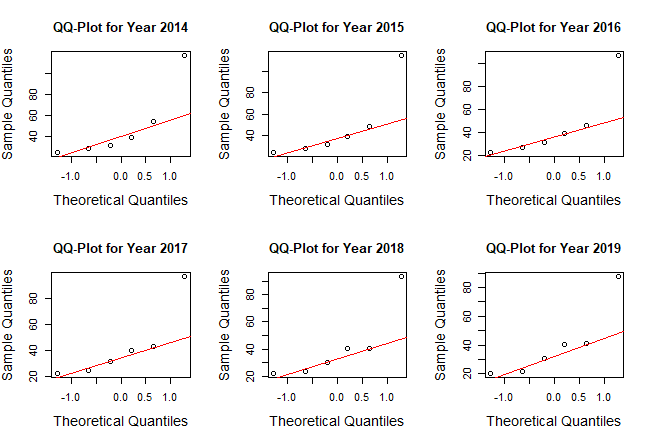
\includegraphics[width=\linewidth]{Images/10 - Thirdqq.png}
	\end{columns}
\end{frame}

\begin{frame}{Quarto gruppo - Paesi con tasso di suicidio più alto per WR}
	\begin{columns}
		\column{0.5\textwidth}
			\begin{itemize}
				\item \textbf{Lesotho} (LSO) per Africa
				\item \textbf{Russian Federation} (RUS) per Europe
				\item \textbf{Somalia} (SOM) per Eastern Mediterranean
			\end{itemize}
			\bigskip
			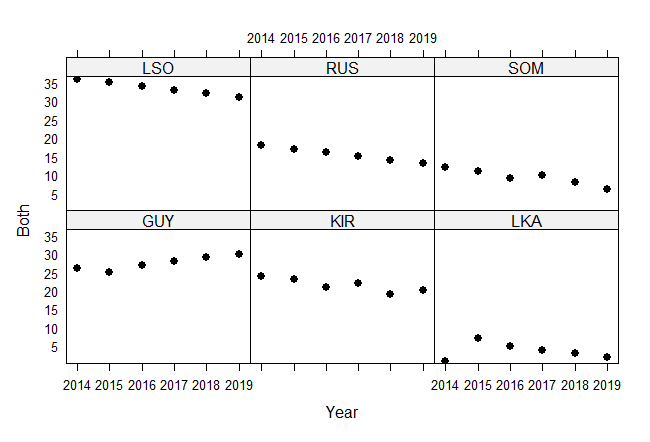
\includegraphics[width=\linewidth]{Images/11 - Fourthgroup.png}
		\column{0.5\textwidth}
			\begin{itemize}
				\item \textbf{Guyana} (GUY) per Americas
				\item \textbf{Kiribati} (KIR) per Western Pacific
				\item \textbf{Sri Lanka} (LKA) per South-East Asia
			\end{itemize}
			\bigskip
			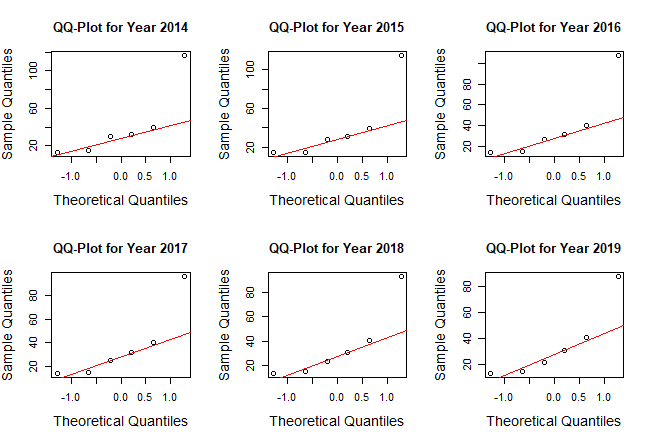
\includegraphics[width=\linewidth]{Images/12 - Fourthqq.png}
	\end{columns}
\end{frame}


\section{Test Statistici} % Section title slide, unnumbered
  
\begin{frame}{Obiettivo dei Test Statistici}
	\begin{itemize}
	  \item \textbf{Obiettivo}: Verificare che i dati, all'interno dei vari gruppi,
	  provengano da distribuzioni che non differiscono
	  in maniera significativa tra di loro.
	  \item \textbf{Strumento}: ANOVA a misure ripetute.
	  \item \textbf{Presupposti}:
		\begin{itemize}
		  \item Verifica della normalità
		  \item Verifica dell'omochedasticità
		  \item Verifica della sfericità
		  \end{itemize}
	  \item Se una di queste assunzioni non è rispettata, si usa il test non parametrico di Friedman.
	\end{itemize}
  \end{frame}

%------------------------------------------------

\begin{frame}{Verifica della normalità}
	\begin{table}[htbp]
		\captionsetup{labelformat=empty} % Rimuovi la dicitura "Table:"
		\caption{Test di Shapiro-Wilk}
		\begin{center}
		\begin{tabular}{|c|c|c|c|c|c|c|}
		\hline
		\textbf{Gruppo}&\multicolumn{6}{|c|}{\textbf{Anni}} \\
		\cline{2-7} 
		 & \textbf{2014} & \textbf{2015} & \textbf{2016} & \textbf{2017} & \textbf{2018} & \textbf{2019}\\
		\hline
		\textbf{1} & 0.531 & 0.672 & 0.690 & 0.705 & 0.708 & 0.719 \\\cline{1-7}
		\textbf{2} & 0.913 & 0.824 & 0.804 & 0.832 & 0.746 & 0.569 \\\cline{1-7}
		\textbf{3} & 0.018 & 0.011 & 0.017 & 0.026 & 0.021 & 0.056 \\\cline{1-7}
		\textbf{4} & 0.015 & 0.011 & 0.018 & 0.037 & 0.046 & 0.071 \\\cline{1-7}
		\hline
		\end{tabular}
		\end{center}
	\end{table}
	Solo i primi due gruppi rispettano il vincolo della normalità.
\end{frame}

\begin{frame}{Verifica dell'omoschedasticità}
	\begin{columns}
		\column{0.45\textwidth}
			\begin{table}[htbp]
				\captionsetup{labelformat=empty} % Rimuovi la dicitura "Table:"
				\caption{Test di Bartlett}
				\begin{tabular}{|c|c|c|}
				\hline
				\textbf{Gruppo} & \textbf{K-squared} & \textbf{p-value} \\
				\hline
				\textbf{1} & 0.27014 & 0.9982 \\\cline{1-3}
				\textbf{2} & 0.39744 & 0.9954 \\\cline{1-3}
				\hline
				\end{tabular}
			\end{table}
		\column{0.45\textwidth}
			\begin{table}[htbp]
				\captionsetup{labelformat=empty} % Rimuovi la dicitura "Table:"
				\caption{Test di Levene}
				\begin{tabular}{|c|c|c|}
				\hline
				\textbf{Gruppo} & \textbf{F-value} & \textbf{p-value} \\
				\hline
				\textbf{3} & 0.037 & 0.9992 \\\cline{1-3}
				\textbf{4} & 0.016 & 0.9999 \\\cline{1-3}
				\hline
				\end{tabular}
			\end{table}
	\end{columns}
	Tutti i gruppi rispettano il vincolo dell'omoschedasticità.
\end{frame}

\begin{frame}{Verifica della sfericità}
	\begin{table}[htbp]
		\captionsetup{labelformat=empty} % Rimuovi la dicitura "Table:"
		\caption{Statistica di Greenhouse-Geisser}
		\begin{center}
		\begin{tabular}{|c|c|}
		\hline
		\textbf{Gruppo} & $\boldsymbol{\varepsilon}$\\
		\hline
		\textbf{1} & 0.2067 \\\cline{1-2}
		\textbf{2} & 0.2280 \\\cline{1-2}
		\textbf{3} & 0.2122 \\\cline{1-2}
		\textbf{4} & 0.2028 \\\cline{1-2}
		\hline
		\end{tabular}
		\label{tab4}
		\end{center}
	\end{table}
	Nessuno dei quattro gruppi
	soddisfa la sfericità, i loro valori $\varepsilon$
	si allontanano troppo da 1.
\end{frame}

\begin{frame}{Test non parametrico di Friedman}
	Non possiamo utilizzare ANOVA, utilizziamo il test di Friedman.
	\begin{table}[htbp]
		\captionsetup{labelformat=empty} % Rimuovi la dicitura "Table:"
		\caption{Test di Friedman}
		\begin{center}
		\begin{tabular}{|c|c|c|}
		\hline
		\textbf{Gruppo} & $\boldsymbol{\chi}$\textbf{-squared} & \textbf{p-value} \\
		\hline
		\textbf{1} & 26.19 & 8.196$\times 10^{-5}$ \\\cline{1-3}
		\textbf{2} & 10.762 & 0.05631 \\\cline{1-3}
		\textbf{3} & 13.143 & 0.02208 \\\cline{1-3}
		\textbf{4} & 8.2857 & 0.1412 \\\cline{1-3}
		\hline
		\end{tabular}
		\label{tab5}
		\end{center}
	\end{table}
	Sono nel secondo e il quarto gruppo abbiamo un p-value $> 0.05$
\end{frame}

\begin{frame}{Analisi Post-hoc}
	Analisi post-hoc sul primo gruppo 
	\begin{table}[htbp]
		\captionsetup{labelformat=empty} % Rimuovi la dicitura "Table:"
		\caption{Test di Wilcoxon con correzione di Benjamini-Hochberg}
		\begin{center}
		\begin{tabular}{|c|c|c|c|c|c|}
		\hline
		\textbf{Anni} & \textbf{2014} & \textbf{2015} & \textbf{2016} & \textbf{2017} & \textbf{2018} \\
		\hline
		\textbf{2015} & 0.438 & - & - & - & - \\ \hline
		\textbf{2016} & 0.108 & 0.043 & - & - & - \\ \hline
		\textbf{2017} & 0.078 & 0.043 & 0.438 & - & - \\ \hline
		\textbf{2018} & 0.043 & 0.043 & 0.043 & 0.043 & - \\ \hline
		\textbf{2019} & 0.043 & 0.043 & 0.043 & 0.043 & 0.043 \\ 
		\hline
		\end{tabular}
		\label{tab6}
		\end{center}
	\end{table}
\end{frame}

\begin{frame}{ANOVA a misure ripetute}
	I primi due gruppi non rispettano esclusivamente il vincolo della sfericità,
	verifichiamo se ANOVA conferma i risultati del test di Friedman
	\begin{table}[htbp]
		\captionsetup{labelformat=empty} % Rimuovi la dicitura "Table:"
		\caption{ANOVA a misure ripetute}
		\begin{center}
		\begin{tabular}{|c|c|c|}
		\hline
		\textbf{Gruppo} & \textbf{F-value} & \textbf{p-value} \\
		\hline
		\textbf{Gruppo 1} & 4.482 & 0.0878 \\\cline{1-3}
		\textbf{Gruppo 2} & 0.229 & 0.652 \\\cline{1-3}
		\hline
		\end{tabular}
		\label{tab7}
		\end{center}
	\end{table}
	In entrambi i casi accettiamo l'ipotesi nulla:
	\begin{itemize}
		\item Nel primo gruppo utilizzando ANOVA accettiamo l'ipotesi nulla per la quale, con Friedman, vi erano fortissime evidenze contrarie
		\item Nel secondo gruppo non abbiamo evidenza contro l'ipotesi nulla, come succedeva con Friedman
	\end{itemize}
	Tuttavia ANOVA è in questo caso molto meno significativo rispetto al test di Friedman!
\end{frame}

\section{Conclusioni}

\begin{frame}{Conclusioni}
	Nell'analisi presentata:
	\begin{itemize}
		\item In alcuni periodi e gruppi specifici (ad es. paesi ad alto PIL e alto tasso di suicidio per WR), non ci sono differenze significative nella distribuzione annuale del tasso di suicidi.
		\item Tuttavia, anche confrontando due gruppi con quattro paesi in comune, ma con due differenze, emergono risultati contrastanti (terzo e quarto gruppo).
		\item Date le diverse cause potenziali del fenomeno, questa analisi fornisce una base per futuri studi che potrebbero integrare questo dataset con altri fattori sociali, economici o geopolitici influenti sulla distribuzione dei tassi di suicidio.
	\end{itemize}
\end{frame}

\appendix

\begin{frame}{Bibliografia}
	\nocite{*} % Display all references regardless of if they were cited
	\begin{thebibliography}{00}
		\bibitem{b1} Shneidman ES. ``The definition of suicide''. New York, NY and London: John Wiley and sons; 1985.
		\bibitem{b2} Gvion Y, Apter A. ``Suicide and suicidal behavior''. Public Health Reviews. 2012;34: epub ahead of print.
		\bibitem{b3} Värnik, P. ``Suicide in the world''. Int. J. Environ. Res. Public Health 2012, 9, 760-771. https://doi.org/10.3390/ijerph9030760 
		\bibitem{b4} World Health Organization. (2023). ``Suicide rates''. Recuperato da https://www.who.int/data/gho/data/themes/mental-health/suicide-rates
		\bibitem{b5} Statistics Canada. (2023). ``Age-standardized rates''. Recuperato da https://www.statcan.gc.ca/en/dai/btd/asr
		\bibitem{b6} countryeconomy.com. (2023). ``GDP - Gross Domestic Product 2019''. Recuperato da https://countryeconomy.com/gdp?year=2019
	\end{thebibliography}
	\bibliographystyle{plain}
\end{frame}


\end{document}
